% aRES_ppi — what the computational work has found so far. Figure-led, deliberately short.
% Build:  latexmk -pdf findings.tex     (or Ctrl+Alt+B in VS Code / LaTeX Workshop)
\documentclass[11pt,a4paper]{article}

\usepackage[T1]{fontenc}
\usepackage[utf8]{inputenc}
\usepackage[margin=2.2cm]{geometry}
\usepackage{graphicx}
\usepackage{xcolor}
\usepackage{booktabs}
\usepackage{array}
\usepackage{float}
\usepackage{amssymb}
\usepackage{caption}
\usepackage{enumitem}
\usepackage[colorlinks=true,linkcolor=navy,urlcolor=navy]{hyperref}

\definecolor{navy}{HTML}{1F4E79}
\definecolor{slotline}{HTML}{B08A00}
\definecolor{slotbg}{HTML}{FFFBEF}
\definecolor{soft}{HTML}{666666}
\definecolor{zn}{HTML}{7B3F9D}

\captionsetup{font=small,labelfont=bf}
\setlength{\parindent}{0pt}
\setlength{\parskip}{5pt}

% --- Empty figure slot: says exactly what to render, how, and where to save it -----------
\newcounter{slot}
\newcommand{\figslot}[4]{%
  \refstepcounter{slot}%
  \par\vspace{4pt}%
  \begin{center}
  \setlength{\fboxsep}{9pt}%
  \fcolorbox{slotline}{slotbg}{%
    \begin{minipage}{0.93\linewidth}
      \textbf{\textcolor{slotline}{$\square$\ Figure slot \theslot{} — #1}}\par\vspace{3pt}
      {\small\textbf{Show:} #2}\par\vspace{2pt}
      {\small\textbf{How:} \texttt{\small #3}}\par\vspace{2pt}
      {\small\textbf{Save as:} \texttt{figs/#4}}\par
      \vspace{10pt}
      {\footnotesize\textcolor{soft}{\dotfill\ replace this box with
       \texttt{\textbackslash includegraphics[width=\textbackslash linewidth]\{figs/#4\}}\ \dotfill}}
    \end{minipage}}
  \end{center}\par\vspace{4pt}%
}

\title{\vspace{-1.2cm}\textbf{aRES — computational findings so far}}
\author{\normalsize Rotation project · \texttt{aRES\_ppi}}
\date{\normalsize\today}

\begin{document}
\maketitle
\vspace{-0.6cm}

Everything below comes from sequence and model analysis only --- no experiment yet. Filled figures
are results; empty slots are renders still to make, each with the exact selection to use.
Open questions are collected in \S6.

\vspace{2pt}
\setlength{\fboxsep}{8pt}
\noindent\fcolorbox{navy}{white}{\begin{minipage}{\dimexpr\linewidth-2\fboxsep-2\fboxrule\relax}
\textbf{In one minute.} Three things the analysis turned up that are not in the paper:
\begin{enumerate}[leftmargin=1.3em,itemsep=1pt,topsep=3pt]
  \item aRES has an \textbf{N-terminal Zn(Cys)$_4$ ribbon} (C8/C11/C31/C34) --- so the N-block is
        two modules, not one, and the PF18870 call starts exactly where the ribbon ends.
  \item The PAE gives a \textbf{clean hinge at residue 122}, which defines the constructs.
  \item \textbf{$\lambda$ has no DNA polymerase} yet aRES defends against it --- so the polymerase
        model cannot be the general rule.
\end{enumerate}
\end{minipage}}

% =====================================================================
\section{Domain architecture}

The AlphaFold3 PAE splits aRES (459 aa) into two blocks with a sharp hinge at residue 122 --- not
into the two domains the annotation suggests.

\begin{figure}[H]
\centering
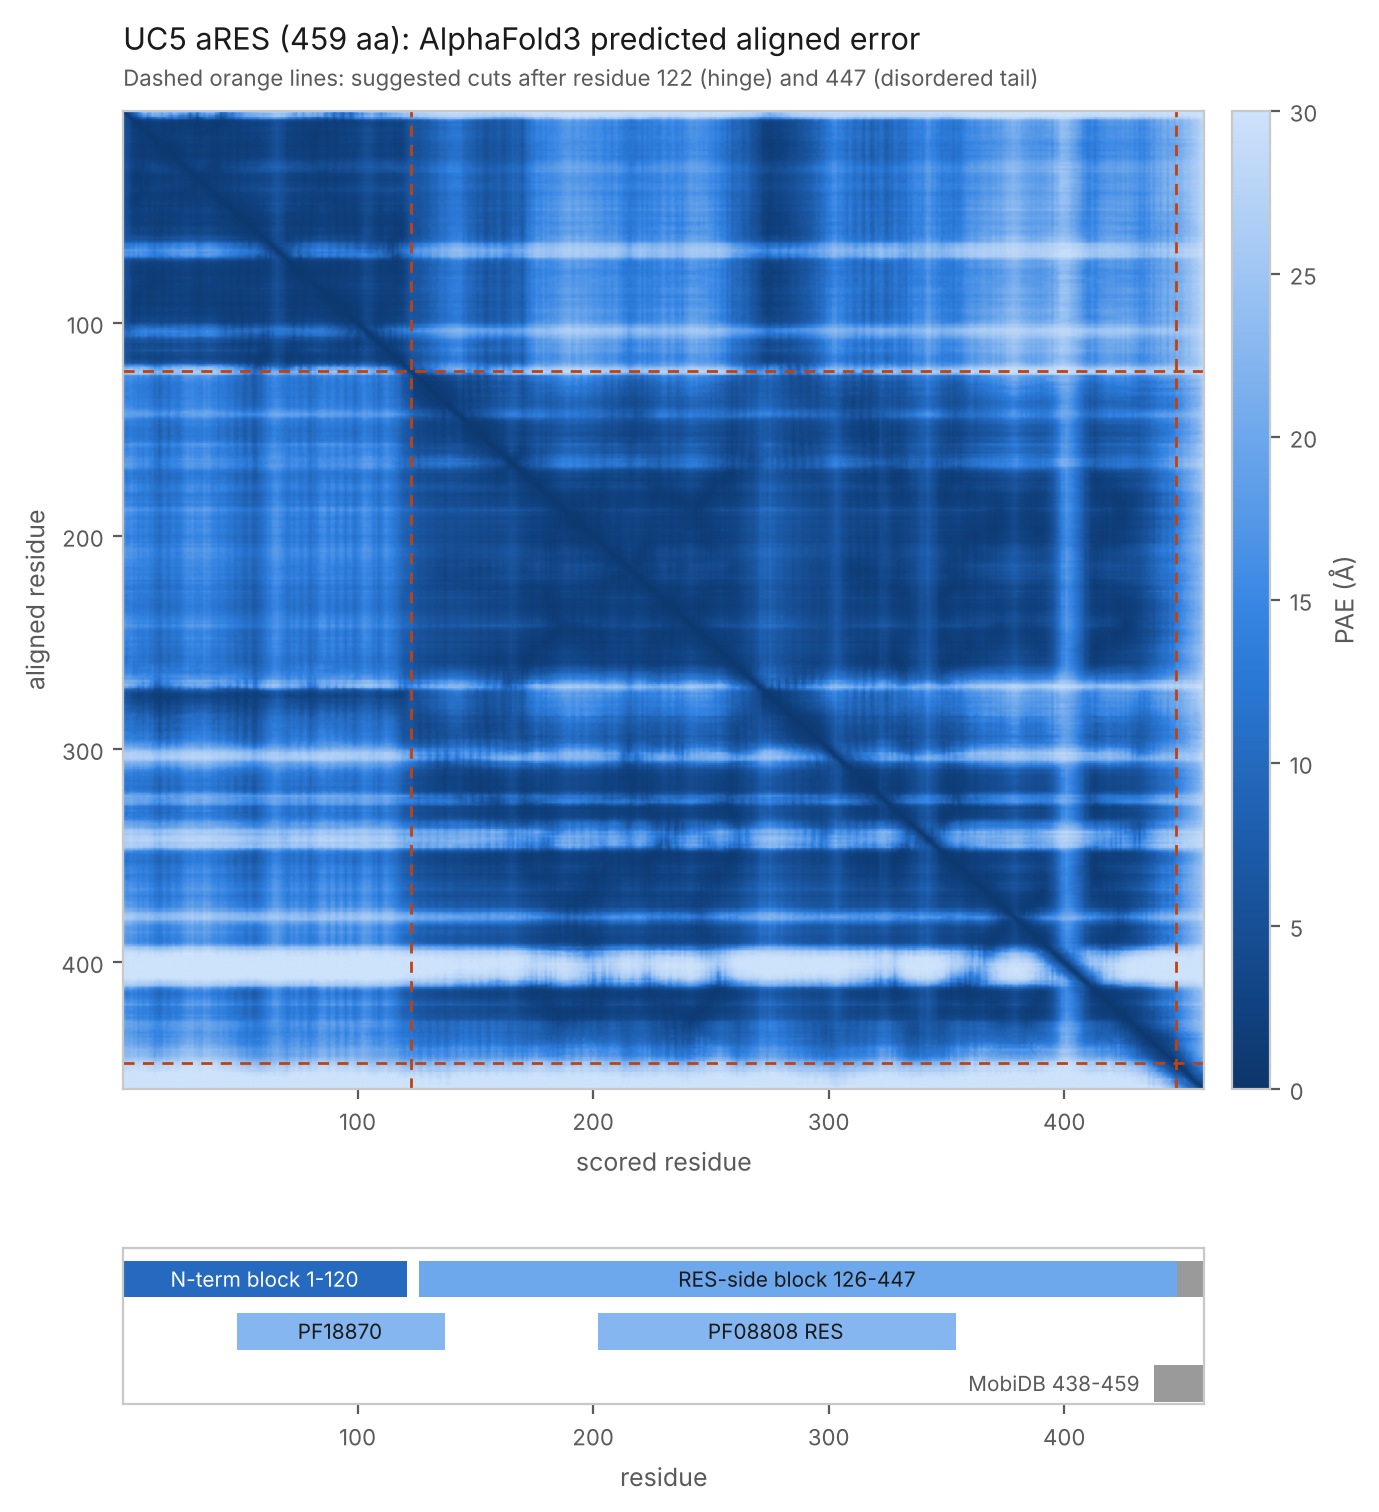
\includegraphics[width=0.56\linewidth]{figs/pae_domains.png}
\caption{UC5 aRES predicted aligned error. Dark blocks are internally confident; the pale cross at
$\sim$122 is the hinge. Residue 123 has PAE 15--17\,\AA{} to \emph{both} sides. The pale band at
392--408 is a flexible loop, and 448--459 is disordered (PAE $>$25\,\AA{} to everything).}
\end{figure}

\begin{center}
\small
\begin{tabular}{@{}llp{0.52\linewidth}@{}}
\toprule
\textbf{Residues} & \textbf{Module} & \textbf{Evidence}\\
\midrule
1--48 & Zn ribbon & Four Cys, tetrahedral (\S3)\\
49--120 & PF18870 / NTD-1 & InterPro calls 49--136; PAE block ends at 120\\
121--125 & \textbf{Hinge} & PAE 15--17\,\AA{} to both sides\\
126--447 & RES-side block & Tight core 171--375 holds R182, R184, E236\\
448--459 & Disordered tail & MobiDB 438--459\\
\bottomrule
\end{tabular}
\end{center}

\textbf{The key point:} the structural N-block (1--120) is \emph{bimodular}. InterPro's PF18870 call
starts at 49 --- exactly where the Zn ribbon ends. The two annotations were never in conflict; they
describe two modules that the PAE saw as one block. Constructs follow the hinge: \textbf{1--120}
(N-block, contains the Zn site), \textbf{126--447} (RES side), \textbf{1--447} (tail trimmed).

% =====================================================================
\section{Pfam accessions}

\begin{figure}[H]
\centering
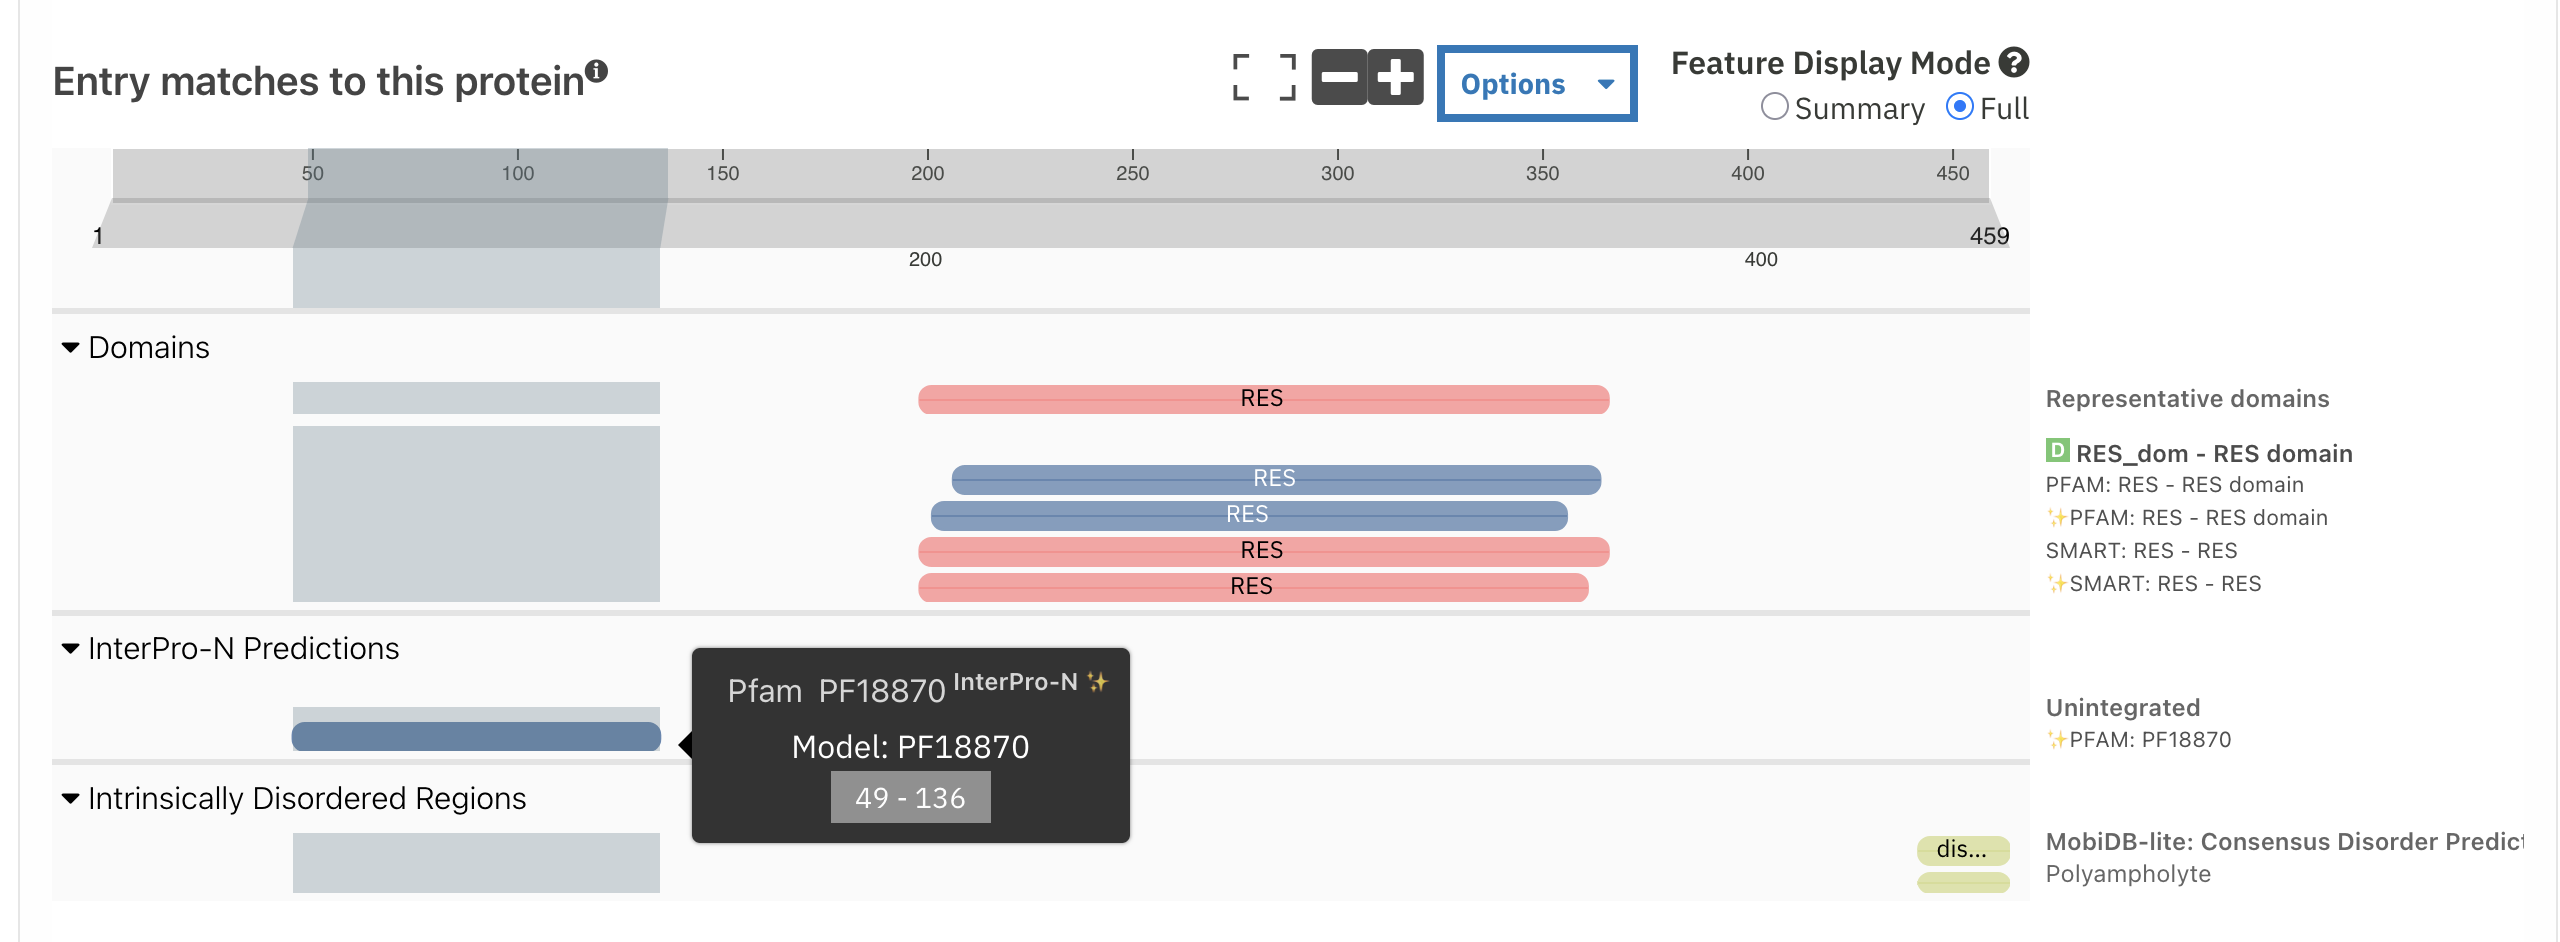
\includegraphics[width=0.97\linewidth]{figs/interpro_domains.png}
\caption{InterPro match for UC5 aRES. PF18870 is an InterPro-N prediction at 49--136; the RES
domain matches sit at $\sim$200--360 from Pfam and SMART.}
\end{figure}

\begin{center}
\small
\begin{tabular}{@{}lllp{0.38\linewidth}@{}}
\toprule
\textbf{Domain} & \textbf{Accession} & \textbf{Range} & \textbf{Note}\\
\midrule
HEPN/RES N-terminal domain 1 & \texttt{PF18870} & 49--136 & No experimental structure of any
PF18870 domain exists anywhere\\
RES NADase & \texttt{PF08808} & 199--363 & See the warning below\\
\bottomrule
\end{tabular}
\end{center}

\textcolor{slotline}{\textbf{Carry-over to check:}} the paper is internally inconsistent about the
RES accession --- Fig.~1B labels it one way, the STAR Methods text another. The wrong accession
returns a histone-like family (CBFD\_NFYB\_HMF), which would silently corrupt an HMM-based homolog
search. Confirm on InterPro before building the alignment. \textbf{Verified so far:}
\texttt{PF18870 = 49--136}, from the screenshot above.

% =====================================================================
\newpage
\section{The Zn(Cys)\texorpdfstring{$_4$}{4} ribbon}

Found by inspecting the aRES model directly --- this was not annotated anywhere. Four cysteines in a
\textbf{CxxC\,\dots\,CxxC} pattern form a tight tetrahedral cluster:

\begin{center}
\small
\begin{tabular}{@{}ll@{}}
\toprule
Cysteines & \textcolor{zn}{\textbf{C8, C11, C31, C34}} \quad (spacing 3, 20, 3)\\
All pairwise SG--SG distances & \textbf{3.55--3.81\,\AA}, mean \textbf{3.67\,\AA}\\
Ideal Zn(Cys)$_4$ edge ($2.3 \times \sqrt{8/3}$) & \textbf{3.76\,\AA} $\rightarrow$ deviation
\textbf{0.09\,\AA}\\
Mean pLDDT of the four Cys & \textbf{90.8} --- confident region, not over-read\\
Not disulfides & an S--S bond is 2.05\,\AA, far shorter\\
Negative control (T7 gp5) & 10 Cys, \textbf{no cluster}; closest pair 7.85\,\AA\\
\bottomrule
\end{tabular}
\end{center}

The other three aRES cysteines (C78, C96, C249) are isolated --- there is no second cluster.
Reproduce with \texttt{python3 analysis/scripts/zn\_site\_check.py <ares\_model.pdb>}.

\figslot{The Zn ribbon}
{The four cysteine side chains as sticks with SG atoms highlighted, the tetrahedron they enclose,
and all six SG--SG distances labelled. Colour C8/C11 and C31/C34 as the two CxxC knuckles so the
ribbon topology is visible. Put the N-block cartoon behind them, transparent.}
{select zn\_cys, resi 8+11+31+34 and name SG; show sticks, byres zn\_cys; distance d1, /A//A/8/SG, /A//A/11/SG \dots{} (all six pairs)}
{zn\_ribbon.png}

\textbf{Three consequences, already fixed in the plan:} never mutate C8/C11/C31/C34 --- they are
folding residues, and a defence-null result there would mean nothing. A 1--120 construct contains
the site, so zinc availability in the buffers matters and strong chelators must be avoided. And
there is \emph{no zinc in the docking model}, only the geometry --- so if docking contacts land on
residues 1--48, discount them until the run is repeated with Zn modelled.

% =====================================================================
\section{The escape-mutant contacts}

Both T7 gp5 escape mutants (\textbf{S122P}, \textbf{D106G}) sit in the same 100--125 loop, which the
blind run narrowed to \textbf{110--118} (R111 and G117 in 28/28 models). Why two chemically unrelated
mutations 16 residues apart give the same phenotype is \textbf{still open}: an earlier two-step
``scaffold and contact'' reading was withdrawn with the cofold pair it was built on.

\textcolor{slotline}{\textbf{Before re-rendering, note the problem with the existing panels:}} the
three PyMOL measurements are not like-for-like --- WT measured OD2(106)$\rightarrow$N(121)
(2.713\,\AA), S122P measured \textbf{CB}(106)$\rightarrow$N(121) (2.777\,\AA), D106G measured
N$\rightarrow$N (6.440\,\AA). The S122P panel measures a carbon with no polar hydrogen, so it is not
reading the H-bond at all. The slots below fix that by using a measure defined in \emph{every}
variant.

\figslot{WT vs.\ S122P vs.\ D106G --- one consistent panel}
{Three aligned sub-panels of the gp5 100--125 loop. In each, label the \emph{same} two measures:
C$\alpha$(106)--C$\alpha$(121) distance, and the 100--125 backbone RMSD to WT. Report the
OD2(106)$\rightarrow$N(121) H-bond separately and only where Asp exists (WT, S122P, S122A) ---
D106G has no side chain, so it cannot have that bond.}
{align mut, wt; distance ca, /A//A/106/CA, /A//A/121/CA; rms\_cur loop\_mut, loop\_wt}
{loop\_wt\_s122p\_d106g.png}

\figslot{The cofold interface}
{The aRES N-block and the gp5 100--125 loop at the predicted interface, with every polar contact
under 3.5\,\AA{} labelled. Mark which aRES residues are in
1--48 (Zn ribbon, discount) versus 49--120 (PF18870, real).}
{sele iface, (chain A within 5 of chain B); distance polar, chain A, chain B, 3.5, mode=2}
{cofold\_interface.png}

\textbf{Treat this interface as provisional, and at domain resolution only.} The specific residue
pair this cofold once nominated has been \textbf{dropped} --- one seed, poor ipTM, and never
reproduced (0/28 docking models, 16\,\AA{} apart). What does not depend on it: the epitope is the
100--125 loop, which comes from phage genetics --- two independently isolated escape mutants, each
escaping both aRES variants --- and the loop faces the N-block rather than the RES domain.

% =====================================================================
\section{What has actually been run}

\begin{center}
\small
\begin{tabular}{@{}p{0.27\linewidth}p{0.30\linewidth}p{0.35\linewidth}@{}}
\toprule
\textbf{Analysis} & \textbf{Result} & \textbf{Status}\\
\midrule
AF3 monomer + PAE & Hinge at 122; block map above & Done, drives the constructs\\
InterPro / Pfam & PF18870 49--136 & Done; RES accession to confirm\\
Zn site scan & Zn(Cys)$_4$ at C8/C11/C31/C34 & Done, with gp5 negative control\\
AF3 cofold aRES\,+\,gp5 & gp5 loop faces the N-block & One seed; its named residue pair is dropped\\
HADDOCK blind run & --- & Output not yet in the repo\\
HADDOCK one-sided restrained & Both escape residues buried & Done; see \texttt{docs/07}\\
Sequence checks & 6 Cys in 1--120; \textbf{no Lys in 49--120} & Done --- constrains amine-reactive
crosslinking directly\\
\bottomrule
\end{tabular}
\end{center}

\textbf{Free and not yet done:} the per-seed audit of the cofold (ipTM, interface PAE, and how often
\emph{any} NTD-1 contact recurs across seeds --- letting the audit nominate contacts rather than
testing a pair chosen in advance). It decides whether the interface in \S4 deserves any further work,
and it needs only the model files, which are not yet in the repo.

\setlength{\fboxsep}{8pt}
\noindent\fcolorbox{navy}{white}{\begin{minipage}{\dimexpr\linewidth-2\fboxsep-2\fboxrule\relax}
\textbf{If I could start two things tomorrow:} the per-seed cofold audit above --- free, and it needs
only the model files --- and the published gp5\,$\Delta$118--123 construct, a catalytically competent
deletion that removes G121/S122 outright. If it still activates aRES, S122 is not the contact. That
is one clone, and it settles \S4.
\end{minipage}}

% =====================================================================
\section{Questions}

\subsection*{On the published data}

\begin{itemize}[leftmargin=1.4em,itemsep=2pt,label=$\square$]
  \item \textbf{Do the escape mutants abolish \emph{binding}, or only \emph{activation}?}
        This is the one that changes the model. If S122P and D106G still bind aRES but no longer
        activate it, then recognition is intact and the defect is in signal transmission --- NTD-1
        would be doing something after binding, not just binding. If they lose binding, the sensor
        model stands as written. The paper has both assays (co-expression toxicity and pull-down),
        so the mutants may already have been run through both.
  \item \textbf{Was the pull-down done with gp5 alone or with the gp5$\cdot$TrxA holoenzyme?}
        The in vitro activation used the commercial holoenzyme. If binding was only ever shown for
        the complex, then thioredoxin cannot be excluded as part of the epitope --- and every
        docking run against gp5 alone is against the wrong species.
  \item \textbf{Is anything known about what triggers aRES in $\lambda$?} $\lambda$ encodes no
        polymerase; its replication proteins are O and P. A candidate reading is that NTD-1 senses
        proteins that \emph{hijack host replication factors} --- gp5 captures thioredoxin, $\lambda$\,P
        captures DnaB. One co-expression panel would test it.
  \item \textbf{Is the aRES sequence in hand the same isolate as the paper's?} The model has Ile234
        and Ser293; the paper's defence-null list says S234A and V293A. That pattern looks like a
        transposed residue pair, and it sits upstream of every mutant.
\end{itemize}

\subsection*{On resources}

\begin{itemize}[leftmargin=1.4em,itemsep=2pt,label=$\square$]
  \item \textbf{Are the AlphaFold cofold files available?} With the coordinates, the per-seed
        interface audit is one command and costs nothing --- and it decides whether the predicted
        contact is worth any further work.
  \item \textbf{Supplementary Tables S2--S4 and Fig.~1B at full resolution?}
  \item \textbf{Does the lab have the aRES constructs (UC5 and S\_34AVR), the escape phage isolates,
        and a gp5$\cdot$TrxA co-expression plasmid?} The commercial enzyme cannot supply the
        quantities needed, and the chimeras have a long cloning lead time, so this sets what can
        start immediately.
  \item \textbf{Access to ICP-MS or native MS for the zinc stoichiometry}, and does the standard
        purification include Zn in the buffers?
\end{itemize}

\subsection*{On direction}

\begin{itemize}[leftmargin=1.4em,itemsep=2pt,label=$\square$]
  \item \textbf{Which is the better use of the rotation:} the \emph{domain} (an apo N-block
        structure --- the first for any PF18870) or the \emph{interaction} (a measured $K_d$ plus an
        interface restraint set)? The domain track has one gate and does not depend on the
        interaction hypothesis being right; the interaction track has four gates but higher value.
  \item \textbf{Has anyone measured the $K_d$?} Every biophysical method has a concentration window,
        so this number decides which are even applicable.
  \item \textbf{Is aRES a monomer?} Assumed everywhere, measured never --- and the only solved
        RES-NADase structure (6GW6) is built on a RES dimer. One SEC-MALS run settles it.
  \item \textbf{How much wet lab is in scope for this rotation}, and what would count as a good
        outcome?
\end{itemize}

\end{document}
